% Flowmatic thesis figure blocks — paste into memoir LaTeX source
% Requires: \usepackage{graphicx} \usepackage{subcaption} \usepackage{float}

% ---------------------------------------------------------------------------
% Chapter 4 — Architecture
% ---------------------------------------------------------------------------

\begin{figure}[H]
  \centering
  
\includegraphics[width=0.92\textwidth]{figures/architecture/01-batch-upload-pipeline.png}
  \caption{Batch upload pipeline implemented in Flowmatic (NestJS + Vue). Authenticated clients upload CSV/JSON; objects persist in S3-compatible storage; asynchronous workers execute quality assessment, cleaning, and optional LLM summarisation before export.}
  \label{fig:batch-upload-pipeline}
\end{figure}

\begin{figure}[H]
  \centering
  
\includegraphics[width=0.92\textwidth]{figures/architecture/02-smart-city-streaming.png}
  \caption{Smart-city streaming pipeline. Simulated or external sensor feeds enter organisation-scoped pipelines; the core unit validates and enriches events; medallion layers and export adapters persist outcomes; optional federated coordination supports distributed training demos.}
  \label{fig:smart-city-streaming}
\end{figure}

\begin{figure}[H]
  \centering
  
\includegraphics[width=0.88\textwidth]{figures/architecture/03-microservices-topology.png}
  \caption{Docker Compose deployment topology: PostgreSQL, MinIO, RabbitMQ, sensor simulator, model-inference service, federated coordinator demo, NestJS backend, and Nginx-served Vue frontend.}
  \label{fig:microservices-topology}
\end{figure}

\begin{figure}[H]
  \centering
  
\includegraphics[width=0.82\textwidth]{figures/architecture/04-medallion-data-lake.png}
  \caption{Medallion data lake layout (bronze, silver, gold) used in the Smart City export stage.}
  \label{fig:medallion-lake}
\end{figure}

% ---------------------------------------------------------------------------
% Chapter 4 — Platform UI (screenshots pending capture)
% ---------------------------------------------------------------------------

\begin{figure}[H]
  \centering
  \fbox{\parbox{0.55\textwidth}{\centering\vspace{1.8cm}\textit{Placeholder: login screenshot}\vspace{1.8cm}}}
  \caption{Flowmatic login interface with organisation-scoped session authentication (screenshot pending).}
  \label{fig:ui-login}
\end{figure}

\begin{figure}[H]
  \centering
  \fbox{\parbox{0.88\textwidth}{\centering\vspace{2.0cm}\textit{Placeholder: batch upload and pipeline runs screenshots}\vspace{2.0cm}}}
  \caption{Tabular data preparation workflow: ingestion and run monitoring for the Astana semi-synthetic dataset (screenshots pending).}
  \label{fig:ui-batch-workflow}
\end{figure}

\begin{figure}[H]
  \centering
  \fbox{\parbox{0.92\textwidth}{\centering\vspace{2.2cm}\textit{Placeholder: smart-city live workbench screenshot}\vspace{2.2cm}}}
  \caption{Live smart-city workbench with simulated sources, WebSocket event stream, and four-stage flow rail (screenshot pending).}
  \label{fig:ui-smart-city-live}
\end{figure}

\begin{figure}[H]
  \centering
  \fbox{\parbox{0.88\textwidth}{\centering\vspace{2.0cm}\textit{Placeholder: core unit and workflow graph screenshots}\vspace{2.0cm}}}
  \caption{Core unit configuration and pipeline topology visualisation (screenshots pending).}
  \label{fig:ui-config-graph}
\end{figure}

% ---------------------------------------------------------------------------
% Chapter 5 — Neural evaluation figures
% ---------------------------------------------------------------------------

\begin{figure}[H]
  \centering
  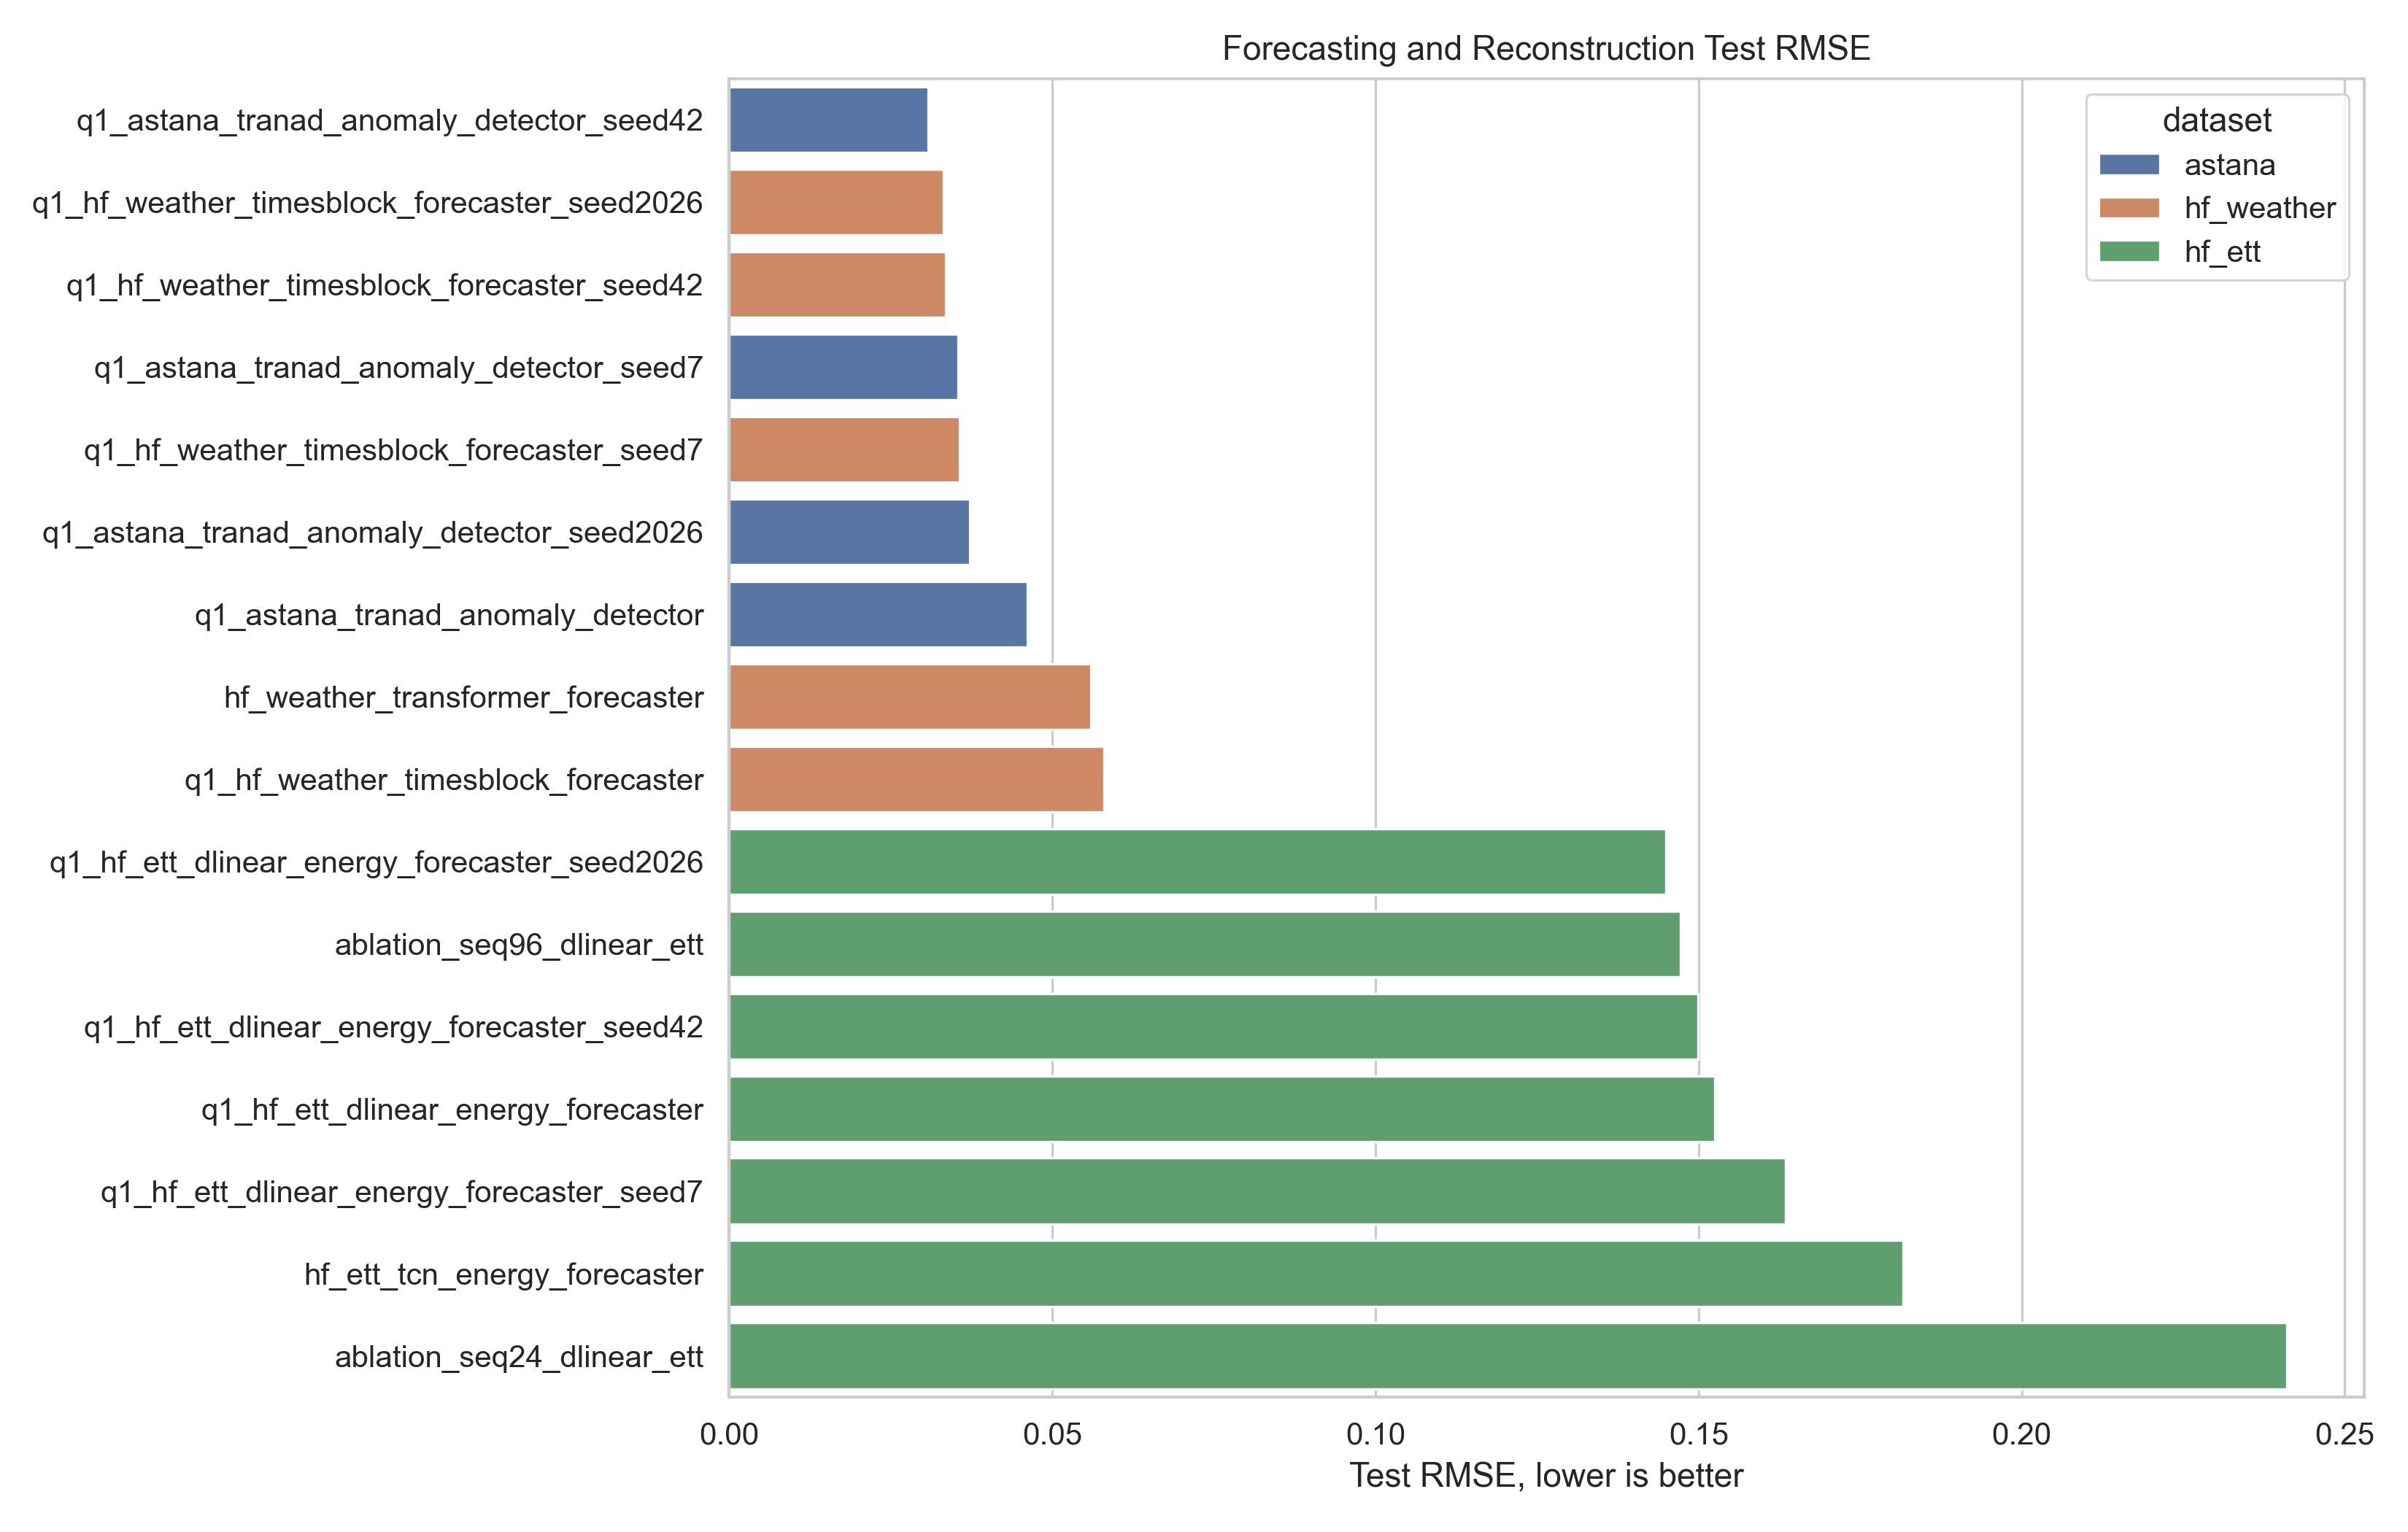
\includegraphics[width=0.85\textwidth]{figures/results/forecast_rmse_leaderboard.png}
  \caption{Neural forecasting and reconstruction leaderboard (test RMSE) across Astana and Hugging Face benchmark bundles.}
  \label{fig:neural-forecast-rmse}
\end{figure}

\begin{figure}[H]
  \centering
  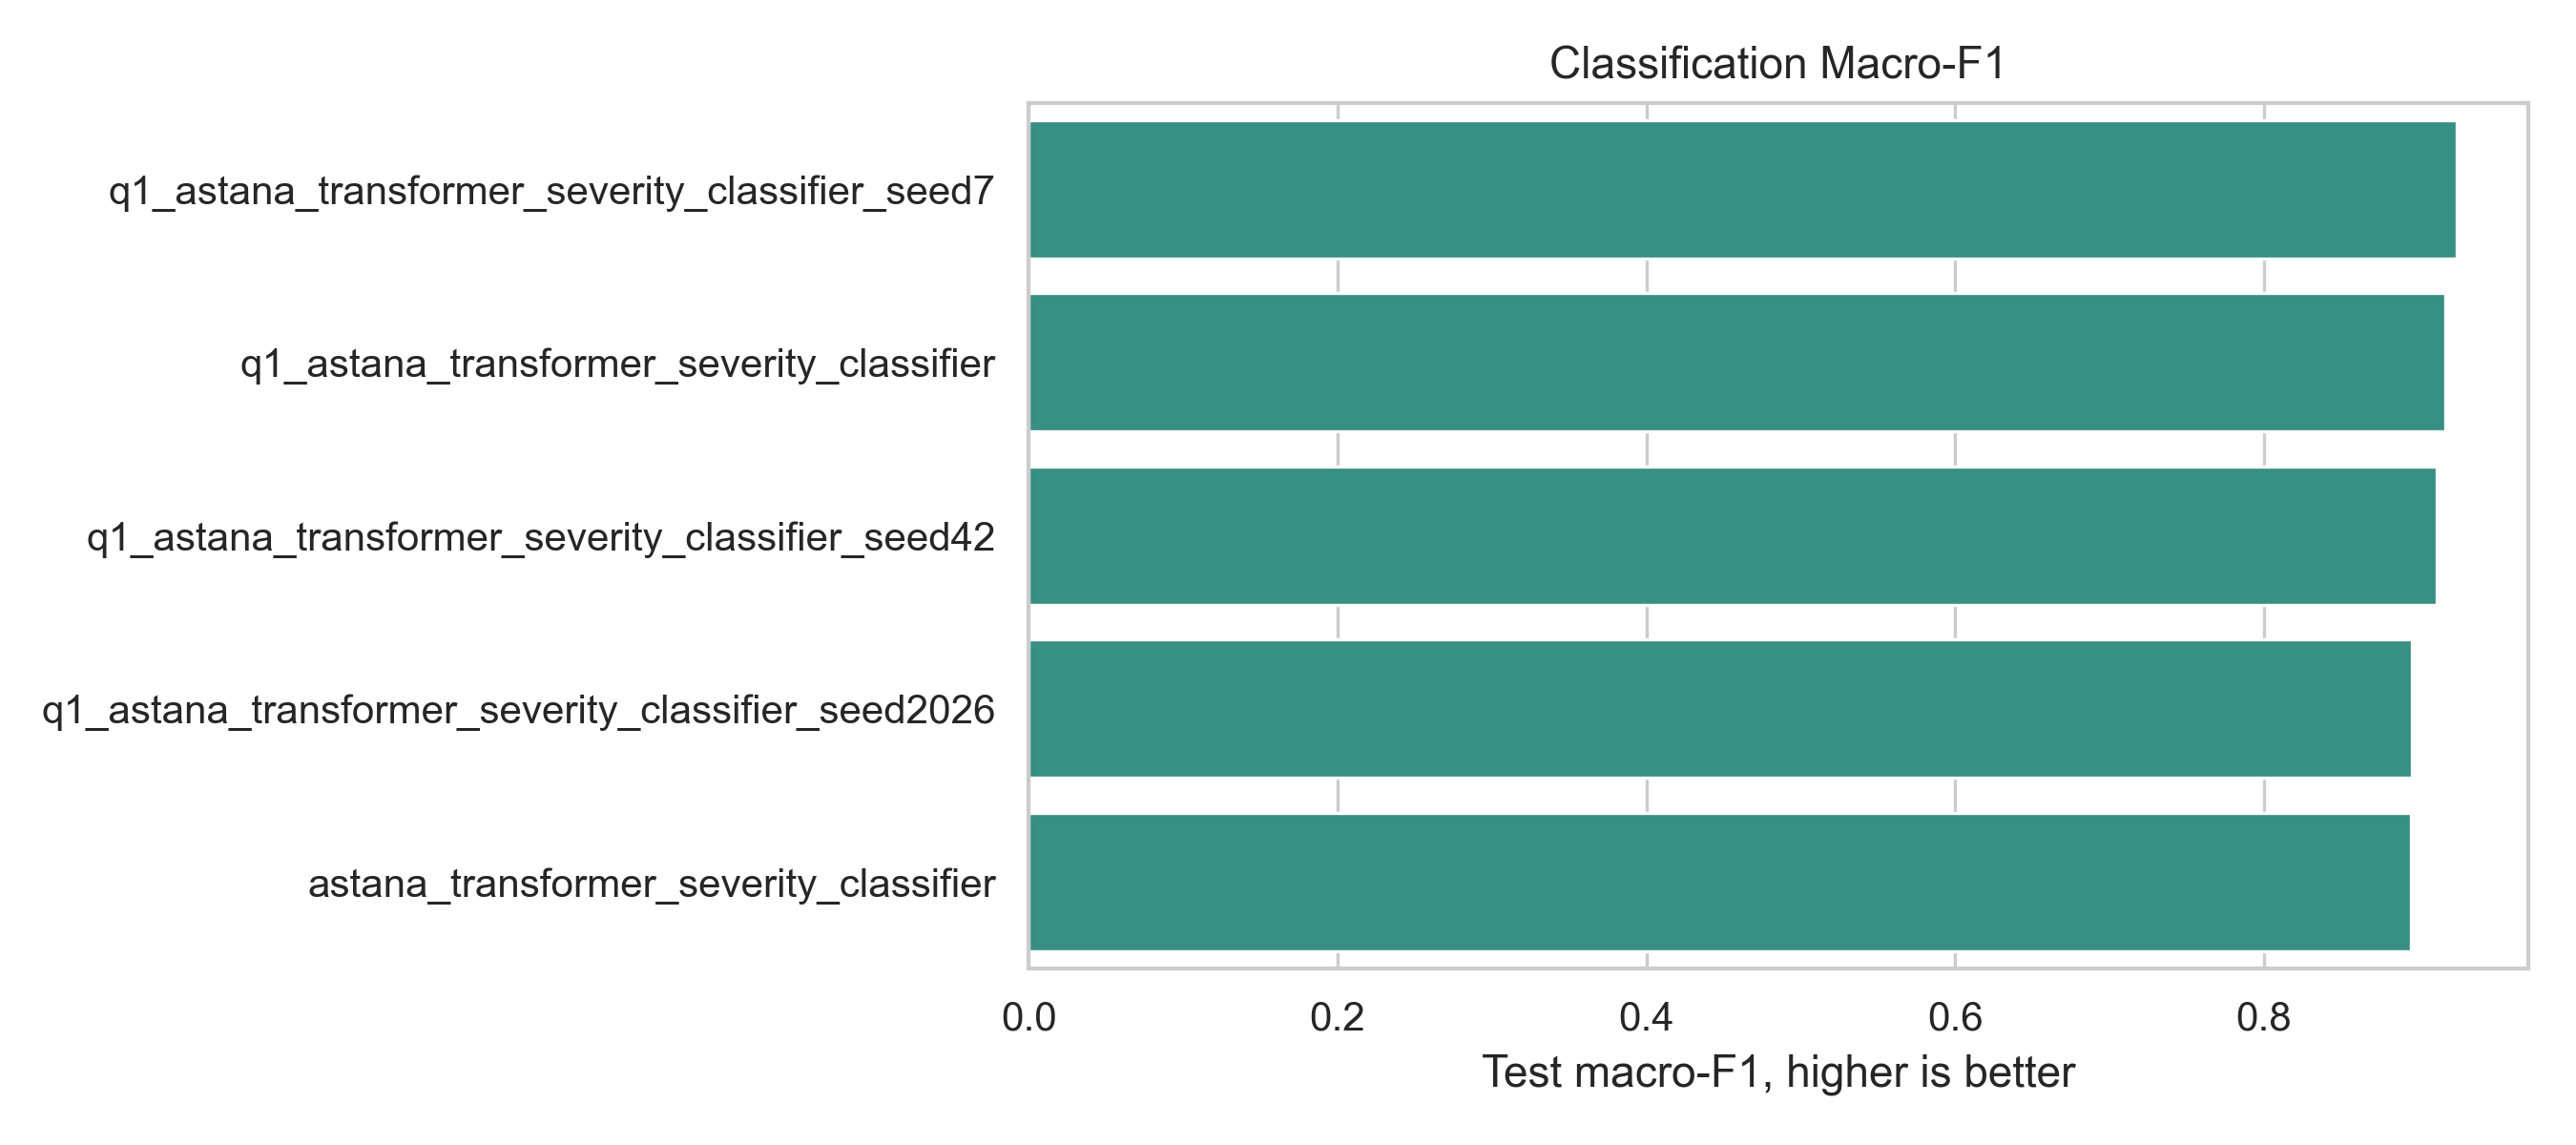
\includegraphics[width=0.85\textwidth]{figures/results/classification_macro_f1.png}
  \caption{Transformer severity classifier macro-F1 compared with classical baselines on Astana traffic events.}
  \label{fig:neural-classification-f1}
\end{figure}

\begin{figure}[H]
  \centering
  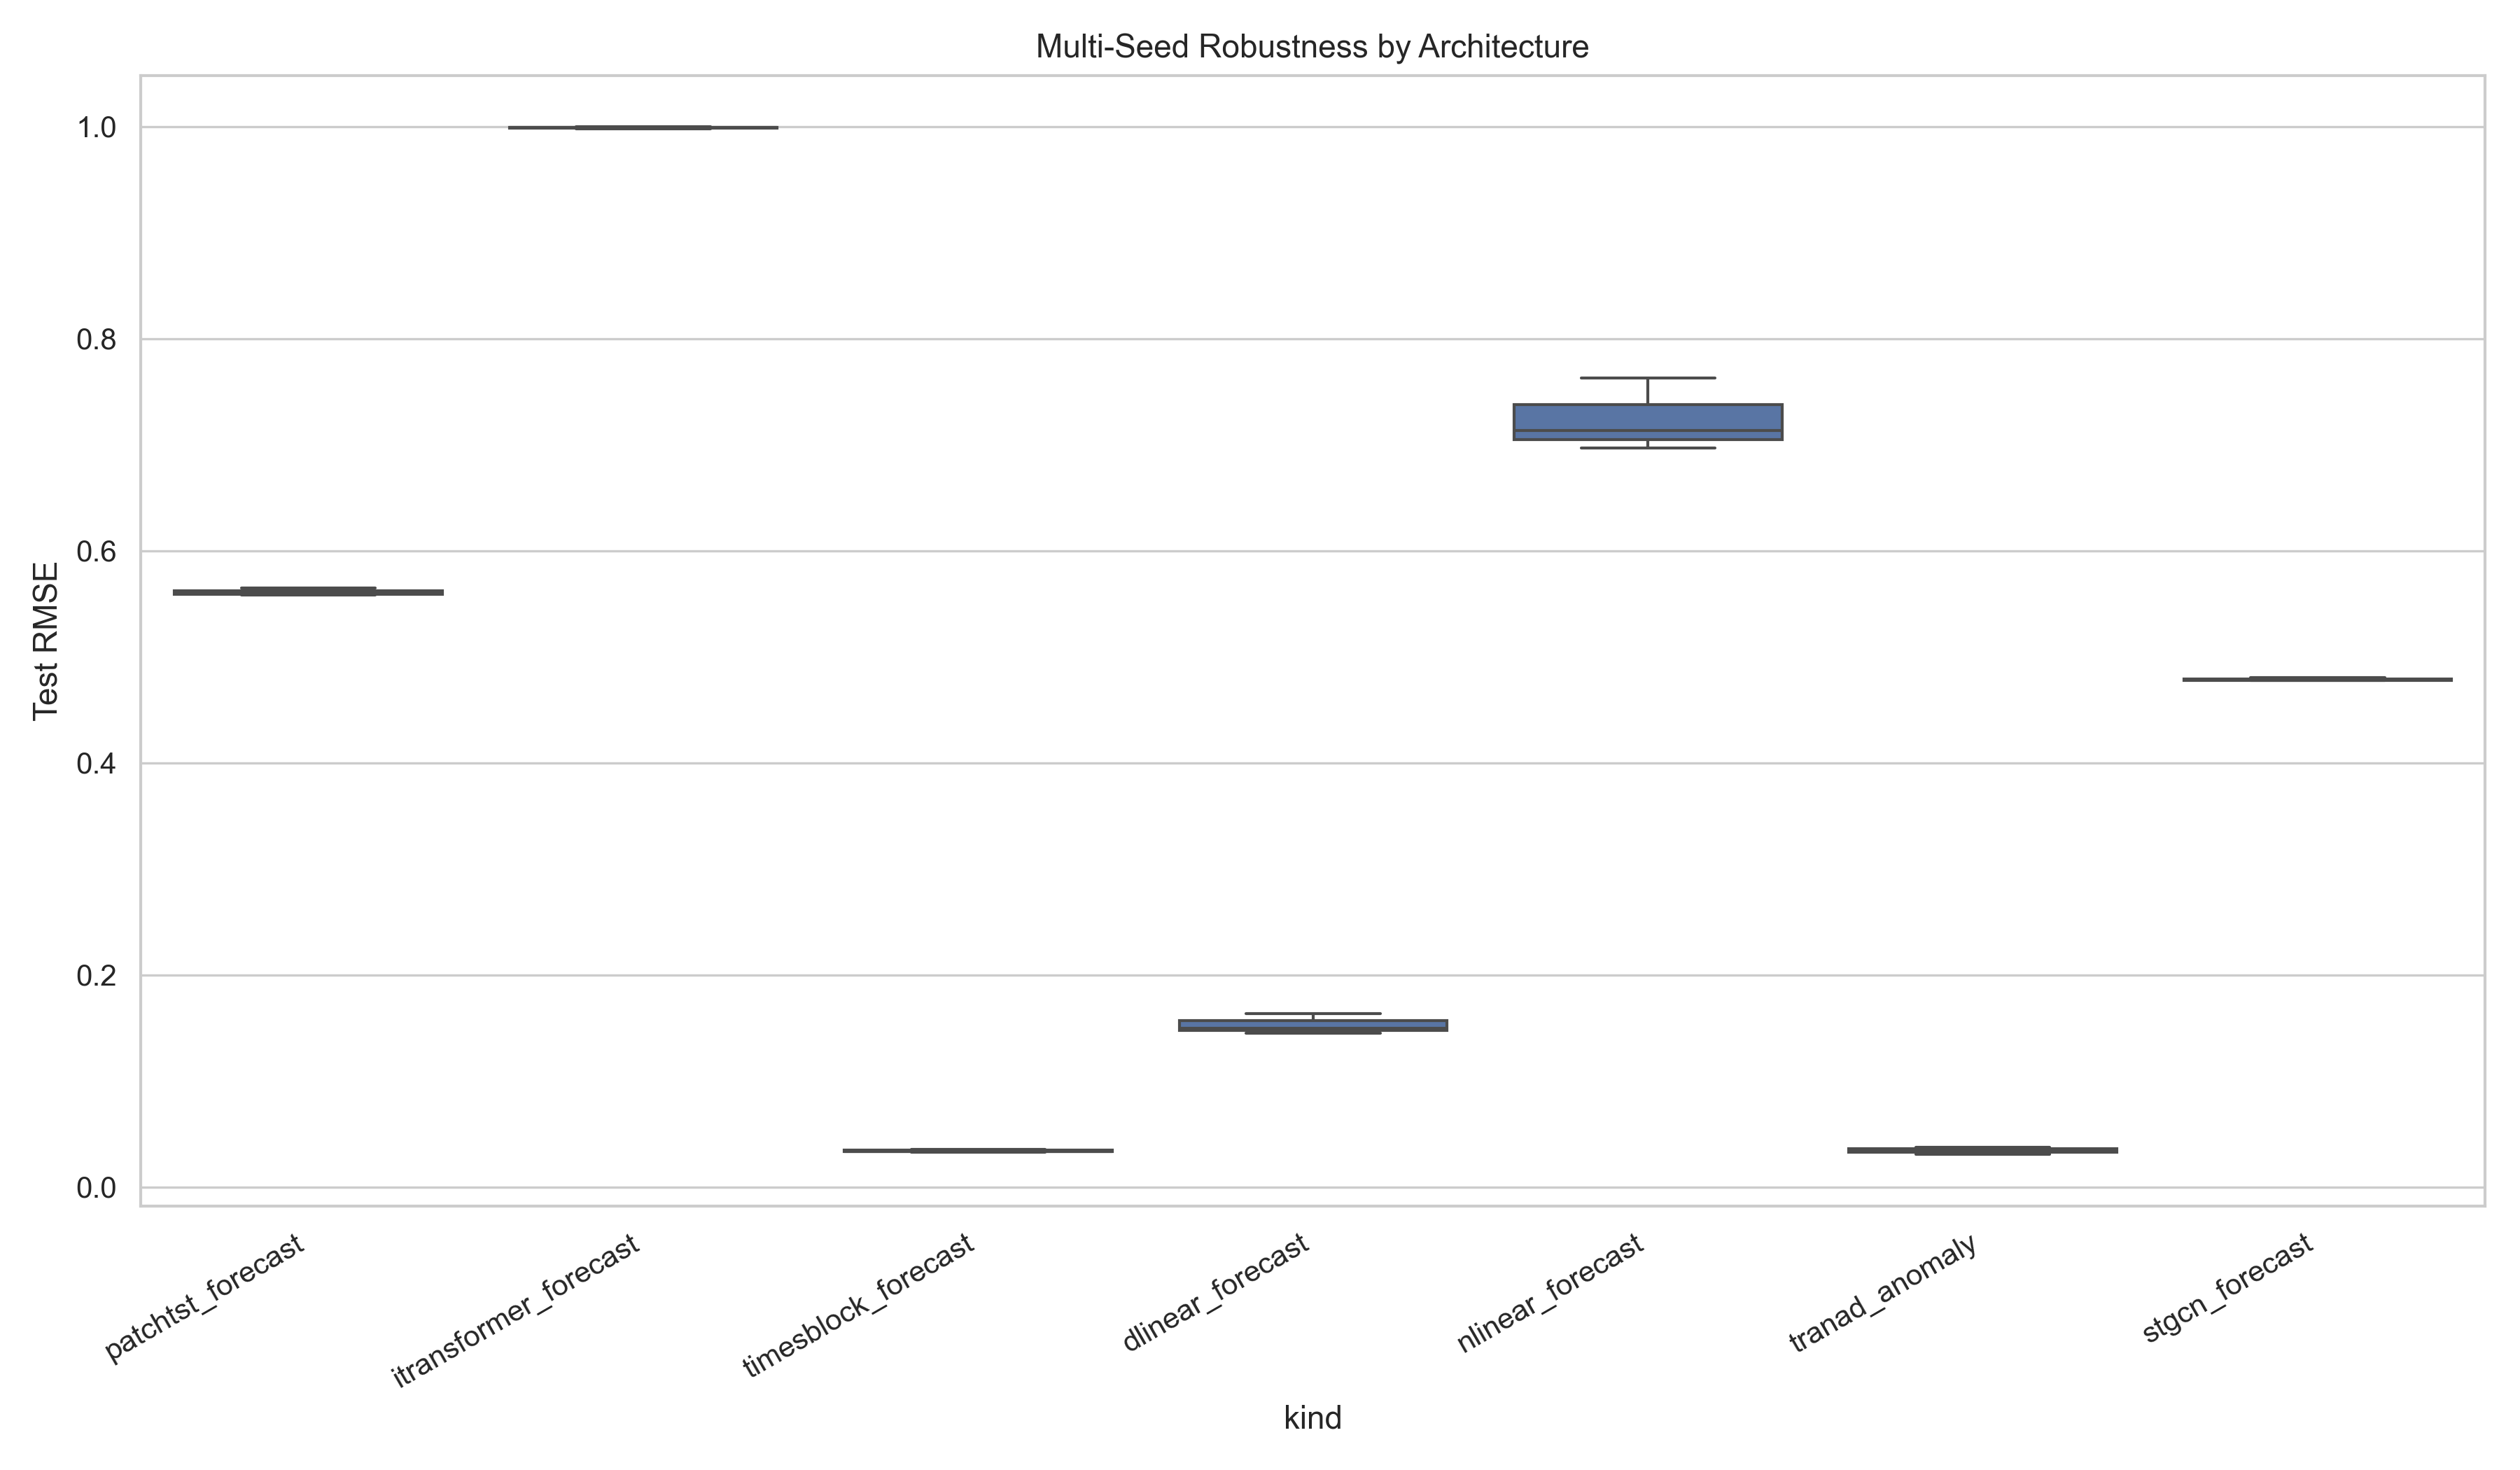
\includegraphics[width=0.85\textwidth]{figures/results/multi_seed_rmse_boxplot.png}
  \caption{Multi-seed robustness (RMSE boxplots) for production portfolio checkpoints.}
  \label{fig:neural-multiseed}
\end{figure}
